%%%%%%%%%%%%%%%%%%%%%%%%%%%%%%%%%%%%%%%%%%%%%%%%%%%%%%%%%%%%%%%
%
% Welcome to Overleaf --- just edit your LaTeX on the left,
% and we'll compile it for you on the right. If you open the
% 'Share' menu, you can invite other users to edit at the same
% time. See www.overleaf.com/learn for more info. Enjoy!
%
%%%%%%%%%%%%%%%%%%%%%%%%%%%%%%%%%%%%%%%%%%%%%%%%%%%%%%%%%%%%%%%
% Author: Izaak Neutelings (Februari 2022)
\documentclass[border=3pt,tikz]{standalone}
\usepackage{physics}
\usepackage{tikz}
\usetikzlibrary{calc}
\usetikzlibrary{patterns}
\usetikzlibrary{arrows.meta} % for arrow size
\usetikzlibrary{decorations.markings}
\tikzset{>=latex} % for LaTeX arrow head

\colorlet{myred}{red!65!black}
\colorlet{mygreen}{green!60!black}
\colorlet{mydarkred}{red!50!black}
\colorlet{mydarkblue}{blue!40!black}
\tikzstyle{measure}=[{Latex[length=4,width=3]}-{Latex[length=4,width=3]},line width=0.4,mydarkblue]
\tikzstyle{ground}=[preaction={fill,top color=black!10,bottom color=black!5,shading angle=20},
                    fill,pattern=north east lines,draw=none,minimum width=0.3,minimum height=0.6]
\tikzstyle{mass}=[line width=0.6,red!30!black,fill=red!40!black!10,rounded corners=1,
                  top color=red!40!black!20,bottom color=red!40!black!10,shading angle=20]
\tikzstyle{rope}=[brown!70!black,line width=1.2,line cap=round] %very thick
\tikzstyle{force}=[->,myred,thick,line cap=round]
\tikzstyle{unit}=[->,mygreen,thick,line cap=round]
\tikzset{fieldlines/.style={mydarkred,decoration={markings,mark=at position #1 with {\arrow{latex}}},
                            postaction={decorate},line width=0.7},
         fieldlines/.default=0.55}
\newcommand{\vbF}{\vb{F}}


\begin{document}


% GRAVITATIONAL ATTRACTION
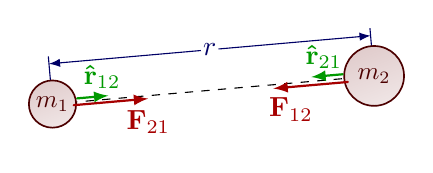
\begin{tikzpicture}
  \def\d{4.1}  % distance r
  \def\r{0.3}  % small radius ball
  \def\R{0.38} % large radius ball
  \def\F{0.95} % force magnitude
  \def\u{0.4}  % unit vector magnitude
  \def\ang{5}  % angle lin
  \coordinate (M1) at (0,0);
  \coordinate (M2) at (\ang:\d);
  
  % SETUP
  \draw[measure,-]
    (M1) --++ (\ang+90:1.6*\R)
    (M2) --++ (\ang+90:1.6*\R);
  \draw[measure] ($(M1)+(\ang+90:1.35*\R)$) --++ (M2)
    node[midway,circle,fill=white,inner sep=0] {$r$};
  \draw[dashed] (M1) -- (M2);
  \draw[mass] (M1) circle(\r) node[scale=0.9] {$m_1$};
  \draw[mass] (M2) circle(\R) node[scale=0.9] {$m_2$};
  
  % FORCES
  \draw[force] (M1)++(\ang-8:0.9*\r) --++ (\ang:\F)
    node[anchor=90,inner sep=4] {$\vbF_{21}$}; % = -G\dfrac{m_1m_2}{r^2}\vu{r}_{21}
  \draw[force] (M2)++(\ang-172:0.9*\R) --++ (\ang:-\F)
    node[anchor=130,inner sep=3] {$\vbF_{12}$}; % = -G\dfrac{m_1m_2}{r^2}\vu{r}_{12}
  \draw[unit] (M1)++(\ang+8:\r+0.02) --++ (\ang:\u)
    node[pos=0.8,above=-1] {$\vu{r}_{12}$};
  \draw[unit] (M2)++(\ang+172:\R+0.02) --++ (\ang:-\u)
    node[pos=0.6,above=-1] {$\vu{r}_{21}$};
  
\end{tikzpicture}


% DROPPING A MASS
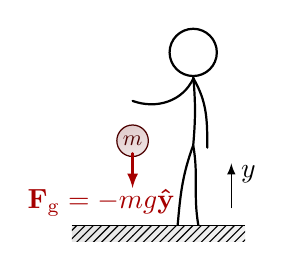
\begin{tikzpicture}
  \def\W{2.2}  % ground width
  \def\D{0.2}  % ground depth
  \def\R{0.2}  % mass radius
  \def\H{2.2}  % human height
  \coordinate (RH) at (-0.15*\W,0.72*\H);
  \coordinate (M) at (-0.15*\W,0.49*\H);
  
  % SETUP
  \draw[ground] (-\W/2,0) rectangle++ (\W,-\D);
  \draw (-\W/2,0) --++ (\W,0);
  \draw[mass,line width=0.45] (M) circle(\R) node[scale=0.8] {$m$};
  
  % PERSON
  \draw[thick] (0.20*\W,\H) circle (0.3) coordinate (H); % head
  \draw[thick] (H)++(-90:0.3) coordinate (N) to[out=-85,in=85]++ (0,-0.40*\H) coordinate (P); % body
  \draw[thick,line cap=round] (N)++(-85:0.03) to[out=-115,in=-20] (RH); % right arm
  \draw[thick,line cap=round] (N)++(-85:0.03) to[out=-60,in=90]++ ( 0.08*\W,-0.4*\H); % left arm
  \draw[thick] (P) to[out=-110,in=85] (0.11*\W,0); % right leg
  \draw[thick] (P) to[out=-80,in=100] (0.23*\W,0); % left leg
  
  % FORCES
  \draw[->] (0.42*\W,0.10*\H) --++ (0,0.26*\H) node[below=4,right=0] {$y$};
  \draw[force] (M)++(0,-0.8*\R) --++ (0,-2.2*\R)
    node[anchor=25,inner sep=0] {$\vbF_\mathrm{g} = -mg\vu{y}$};
  
\end{tikzpicture}


% MASS ON A SURFACE
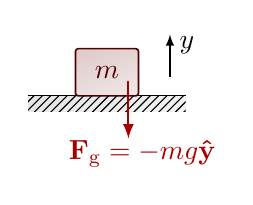
\begin{tikzpicture}
  \def\W{2.0} % ground width
  \def\D{0.2} % ground depth
  \def\h{0.6} % mass height
  \def\w{0.8} % mass width
  \draw[ground] (-\W/2,0) rectangle++ (\W,-\D);
  \draw (-\W/2,0) --++ (\W,0);
  \draw[mass] (-\w/2,0) rectangle++ (\w,\h) node[midway] {$m$};
  \draw[->] (1.0*\w,0.4*\h) --++ (0,0.9*\h) node[below=4,right=0] {$y$};
  \draw[force] (0.34*\w,0.3*\h) --++ (0,-1.2*\h)
    node[right=5,below=-3] {$\vbF_\mathrm{g} = -mg\vu{y}$};
\end{tikzpicture}


% GRAVITATIONAL FORCE FIELD of Earth
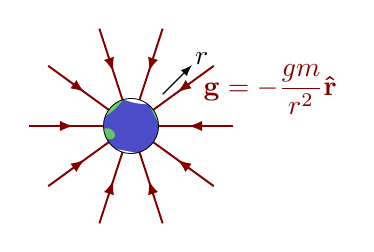
\begin{tikzpicture}
  \def\W{2.4}   % ground width
  \def\D{0.2}   % ground depth
  \def\H{1.5}   % height
  \def\E{0.35}  % Earth's radius
  \def\R{1.3}   % field line max. radius
  \def\N{10}    % number of field lines
  \def\rang{45} % angle or r axis
  
  % FIELD LINES
  \foreach \i [evaluate={\ang=\i*360/\N;}] in {1,...,\N}{
    \draw[fieldlines=0.6] (\ang:\R) -- (\ang:\E); % field lines
  }
  \node[mydarkred,right] at (30:0.71*\R) {$\vb{g} = -\dfrac{gm}{r^2}\vu{r}$};
  \draw[->] (\rang:0.44*\R) --++ (\rang:0.4*\R) node[anchor=\rang+170,inner sep=1] {$r$};
  
  % EARTH
  \fill[blue!70!black!70] (0,0) circle(\E);
  \begin{scope}[rotate=-11]
    \clip (0,0) circle(\E);
    \fill[white] (0,\E) ellipse({0.6*\E} and {0.15*\E});
    \fill[white] (0,-\E) ellipse({0.8*\E} and {0.08*\E});
    \fill[green!70!black!60,rotate=-30] (160:1.1*\E) ellipse({0.2*\E} and {0.8*\E});
    \fill[green!70!black!60,rotate=40] (-10:1.14*\E) ellipse({0.2*\E} and {0.9*\E});
    \fill[green!60!black!60,very thick,rotate=-20] % Australia
      (230:0.86*\E) ellipse({0.25*\E} and {0.18*\E});
  \end{scope}
  \draw[line width=0.3] (0,0) circle(\E);
  
\end{tikzpicture}


% GRAVITATIONAL FORCE FIELD on Earth's surface
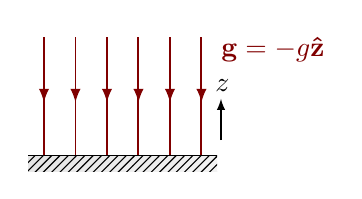
\begin{tikzpicture}
  \def\W{2.4} % ground width
  \def\D{0.2} % ground depth
  \def\H{1.5} % height
  \def\N{6}   % number of field lines
  \draw[->] (1.02*\W,0.13*\H) --++ (0,0.35*\H) node[right=0.5,above=-1] {$z$};
  \node[mydarkred,right=-2] at (\W,0.9*\H) {$\vb{g} = -g\vu{z}$};
  \foreach \i [evaluate={\x=(\i-0.5)*\W/\N;}] in {1,...,\N}{
    \draw[fieldlines] (\x,\H) -- (\x,0); % field lines
  }
  \draw[ground] (0,0) rectangle++ (\W,-\D);
  \draw (0,0) -- (\W,0);
\end{tikzpicture}


\end{document}